This section presents the implementation of the theory in Python and Rust code and the results of various analyses. Unless stated otherwise, all the results were produced using $45'360$ samples (a highly composite number, see \cite{wikipedia_highly_composite_number}).
\section{Details about the Implementation}\label{sec: implementations}
The code can be found under the following link:
\begin{center}
    \url{https://github.com/FiPf/LFT/tree/main/Final%20Project}
\end{center}
All of the code is in the subfolder "Final Project", please ignore all the other subfolders.
\subsection{Description of the Python Code}
The Python code is split into various subfolders, which serve as packages: 
\begin{itemize}
    \item \textbf{algorithms:} This package contains an abstract base class to run simulations with an unspecified algorithm. There are two classes (for Metropolis and HMC), which inherit from this abstract base class and are used to run Metropolis and HMC simulations. Finally, there is a file containing the two integrator choices for the HMC algorithm (leapfrog or omelyan2 integrator). 
    \item \textbf{physics:} This file contains all functions regarding the physics of this project. The first file contains the action of the $\phi^4$-theory, its derivative, a function to calculate the hamiltonian of the system and an enum with the boundary condition choices (either periodic or aperiodic).
    \item \textbf{stats:} This package contains a file with all the statistical analysis functions used for this project. The file intended for logging is currently empty, but the code could be extended to contain loggers. 
    \item \textbf{Main Notebook: }The main file is a Jupyter Notebook, where all of the results are displayed. It accesses the other files through the packages described above. To get an overview, first have a look at this Jupyter notebook.
\end{itemize}
\subsection{Description of the Rust Code}
As shown in Section \ref{sec: data_runtime}, the HMC algorithm was extremely slow in Python, despite most computations being vectorized. It is possible that the object oriented structure of the code contributes to the slowness. Since rewriting the code in a faster way would be a considerable effort and only lead to a small improvement, I decided to instead translate the slowest parts into Rust. \\
Rust is much faster than Python, because Rust is a compiled ahead-of-time to machine code, while Python is an interpreted language (bytecode executed by the CPython virtual machine). This alone can lead to a speedup of a factor $10-100x$. Rust also has other useful features that make coding typesafe and less chaotic than in Python. \cite{rust_cookbook}\\\\
The following parts of the code were translated from Python to Rust: 
\begin{itemize}
    \item The HMC algorithms, together with the two integrators. 
    \item The Metropolis algorithm. 
    \item Some of the physics functions, for example the action and gradient, as they were used for HMC.
\end{itemize}
The structure was kept similar to the Python version. I used PyO3 to be able to import the Rust functions as a package and then use inside my Jupyter Notebook, together with Python code for analysis and plotting. \cite{pyo3}\\\\
Note that translating alone can lead to a great speedup. Since I am still learning Rust, this was a pure translation exercise. I did not use any special features of Rust or payed attention to writing efficient code. Likely, a greater speed-up could be achieved by doing so. 
\section{Tuning the Algorithms to the Correct Acceptance Rate}\label{sec: tuning}
In the Metropolis algorithm, the proposal step size is tuned to achieve an acceptance rate of approximately 50\%. This value represents a compromise between making sufficiently large moves in configuration space and maintaining a reasonable probability of acceptance. If the acceptance rate is too high, the proposed updates are very small and the Markov chain explores the configuration space inefficiently. If it is too low, most proposals are rejected and the simulation again becomes inefficient. \\\\
In contrast, the HMC algorithm is based on approximate Hamiltonian dynamics, where rejections arise solely from numerical integration errors. Since each HMC proposal involves a full molecular dynamics trajectory, rejected updates are computationally expensive. For this reason, HMC is optimally operated at much higher acceptance rates, typically around 90\%. Higher acceptance ensures accurate energy conservation and efficient exploration of phase space, especially when using higher-order integrators such as the omelyan2 scheme. \\\\
\begin{figure}[H]
    \centering
    \begin{subfigure}[b]{0.48\linewidth}
        \centering
        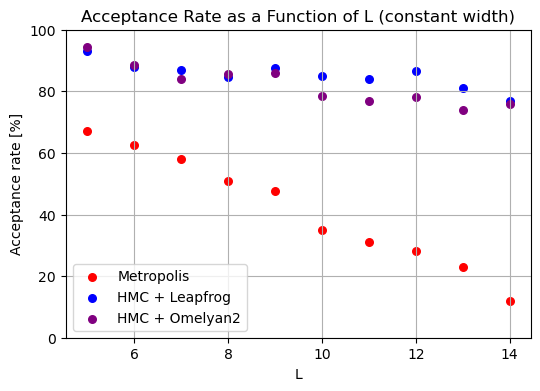
\includegraphics[width=\linewidth]{images/acc_rate_constant_width.png}
        \caption{The dependence of the acceptance rate on the lattice size $L$. The following widths were used: Metropolis w = 0.14 / HMC + Leapfrog w = 0.2 / HMC + Omelyan2 w = 0.44}
        \label{fig:const_width}
    \end{subfigure}
    \hfill 
    \begin{subfigure}[b]{0.48\linewidth}
        \centering
        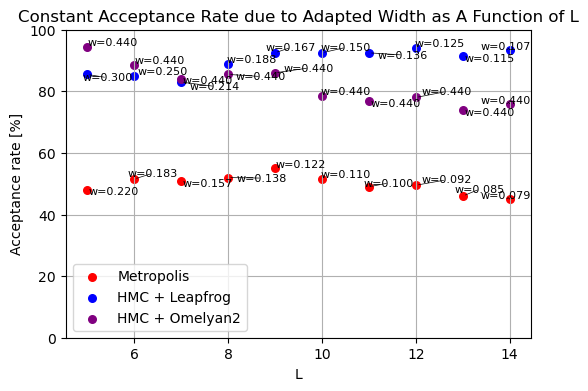
\includegraphics[width=\linewidth]{images/acc_rate_adapted.png}
        \caption{The widths were adapated as a function of $L$ to achieve an acceptance rate of 50\% for Metropolis and 90\% for HMC. The following width functions were used: Metropolis w = 1.1/L / HMC + Leapfrog w = 1.5/L / HMC + Omelyan2 w = 0.44 (const). }
        \label{fig:adapted_width}
    \end{subfigure}
    \caption{Tuning the Acceptance Rates for Different Algorithms}
    \label{fig:tuning_the_acceptance_rates}
\end{figure}
The same tuning parameters were also applied in the Rust implementation. This served as a consistency check to ensure that the Rust version produces results comparable to the Python version.
\section{Monte Carlo Chain Visualization}\label{sec:chain_visual}
In Figure \ref{fig:MC chain}, the Monte Carlo chain of the simulation with different algorithms is shown. The observable displayed is the mean field. These plots are not very useful.
\begin{figure}[H]
    \centering
    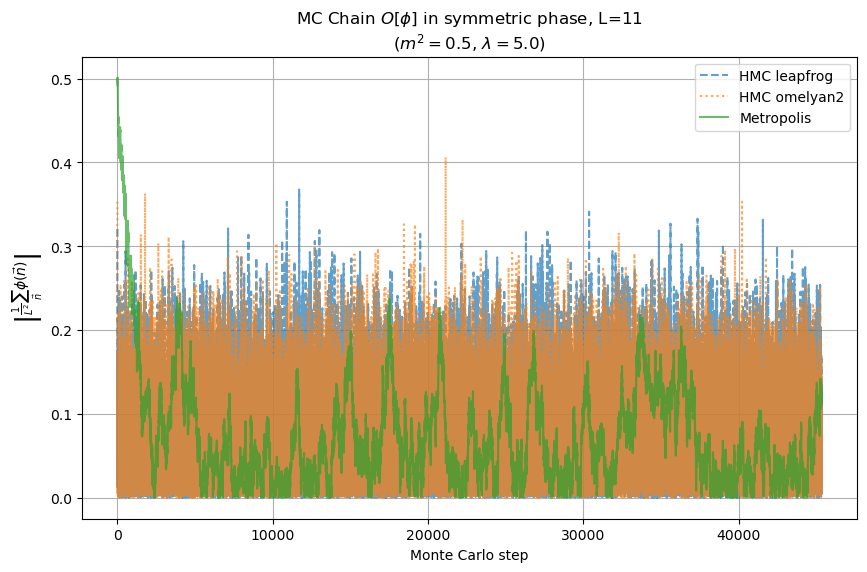
\includegraphics[width=\linewidth]{images/chain.png}
    \caption{Monte Carlo Chain of the Mean Field, Simulation using Different Algorithms}
    \label{fig:MC chain}
\end{figure}
The Metropolis algorithm has the longest thermalization phase, as indicated by the initial drift of the mean field before reaching equilibrium. In contrast, the HMC simulations thermalize more rapidly, likely due to the global updates.
\section{Computational Performance of the Algorithms}\label{sec: data_runtime}
In this section, the computational performance of the different simulation algorithms is compared. The runtimes are shown as a function of lattice size. In addition, the impact of the programming language is investigated comparing Python and Rust versions of the same algorithm. Since lattice simulations are limited by the computational cost, choosing the right algorithm and programming language is crucial. \\\\
The Metropolis and HMC algorithms differ also in their structure and in where most of the computational cost is concentrated. While Metropolis updates are local and inexpensive per step, they suffer from long autocorrelation times. HMC, on the other hand, performs global updates using molecular dynamics trajectories, which are computationally more expensive per iteration but typically yield much faster decorrelation. The statistical independence between configurations is investigated in Section \ref{sec: errs}. \\\\
Furthermore, Python and Rust differ fundamentally in other aspects. Python offers ease of implementation and flexibility but incurs significant overhead due to interpretation and dynamic typing. In contrast, Rust compiles to optimized native code and allows exact control over memory and numerical operations, making it well suited for computationally intensive simulations. In this final project, the computationally intensive algorithms were implemented in Rust and then imported to Python using PyO3 (see \cite{pyo3}). This allows to still use the wonderful Python libraries such as numpy and matplotlib for the analysis and plotting. \\\\
Figures \ref{fig:Pythonruntimes} show the runtimes for the different algorithms in the broken and in the symmetric phase of $\phi^4$-theory using the algorithms implemented in Python. 
\begin{figure}[H]
    \centering
    \begin{subfigure}[b]{0.48\linewidth}
        \centering
        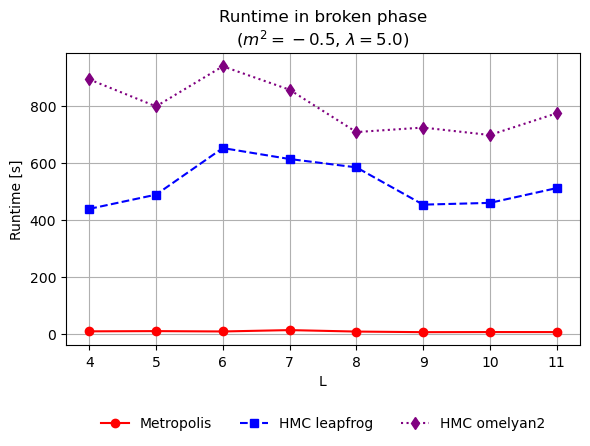
\includegraphics[width=\linewidth]{images/runtimes_Python_broken.png}
        \caption{Broken phase with negative mass}
        \label{fig:broken_python_rt}
    \end{subfigure}
    \hfill 
    \begin{subfigure}[b]{0.48\linewidth}
        \centering
        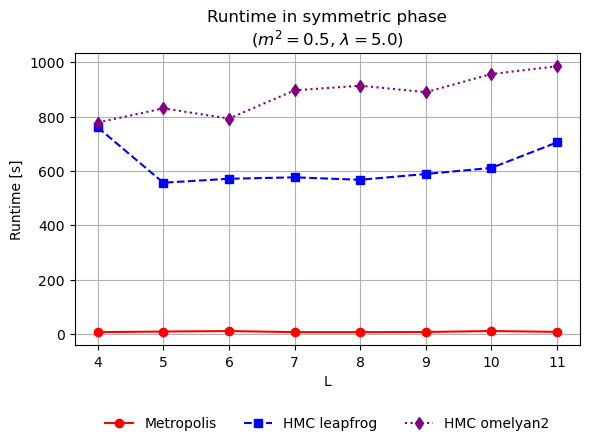
\includegraphics[width=\linewidth]{images/runtimes_Python_symmetric.png}
        \caption{Symmetric phase with positive mass}
        \label{fig:symmetric_python_rt}
    \end{subfigure}
    \caption{Python runtimes}
    \label{fig:Pythonruntimes}
\end{figure}
Figures \ref{fig:Rustruntimes} show the runtimes for the different algorithms in the broken and in the symmetric phase of $\phi^4$-theory using the algorithms implemented in Rust. 
\begin{figure}[H]
    \centering
    \begin{subfigure}[b]{0.48\linewidth}
        \centering
        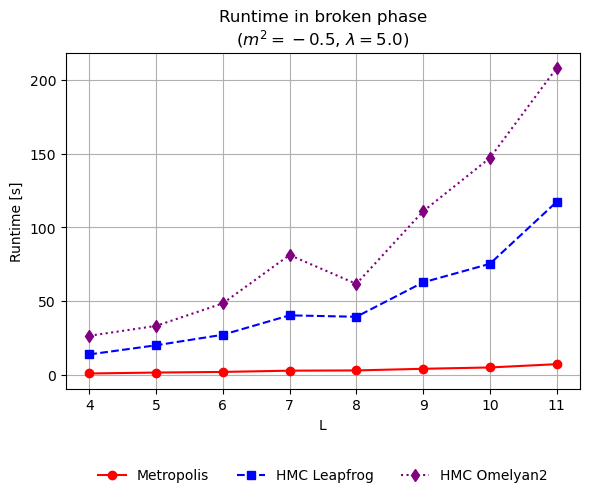
\includegraphics[width=\linewidth]{images/runtimes_Rust_broken.png}
        \caption{Broken phase with negative mass}
        \label{fig:broken_rust_rt}
    \end{subfigure}
    \hfill 
    \begin{subfigure}[b]{0.48\linewidth}
        \centering
        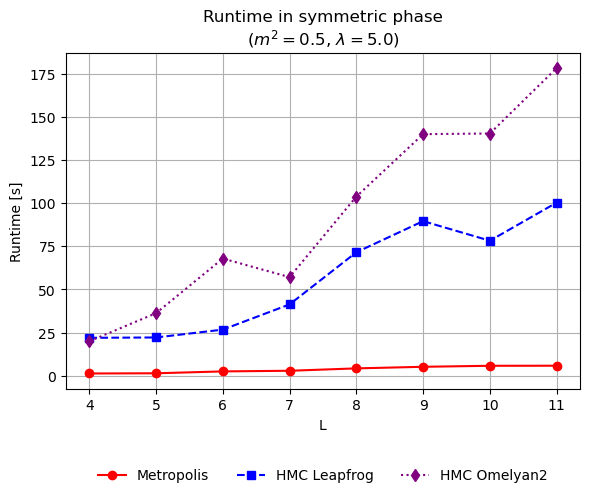
\includegraphics[width=\linewidth]{images/runtimes_Rust_symmetric.png}
        \caption{Symmetric phase with positive mass}
        \label{fig:symmetric_rust_rt}
    \end{subfigure}
    \caption{Rust runtimes}
    \label{fig:Rustruntimes}
\end{figure}
\subsubsection*{Comments on the Results}
\begin{itemize}
    \item Very clearly visible is the speedup achieved by translating the Python code into Rust, the Rust runtimes are a factor of $4-6x$ faster. This was achieved by translating to a more suitable programming language, no efficiency improvements in the algorithms were implemented.
    \item The Metropolis algorithm is the fastest overall, in both Python and Rust. In the Python implementation, the runtime of Metropolis is nearly constant, while in Rust, we observe a slight increase with increasing lattice size $L$. 
    \item The HMC algorithm is significantly slower than the Metropolis algorithm, where the leapfrog integrator is faster than the omelyan2 integrator used in HMC. 
    \item In the Python version, the runtime of HMC for both integrators are more or less constant with the lattice size $L$ for unclear reasons. For the Rust versions of the HMC algorithms, we observe a linear increase of runtime with $L$. This can be explained by the fact that HMC has a larger configuration to update and the equations of motion are more expensive to solve. 
    \item In addition, it can be observed that the runtime in the symmetric phase is higher than in the broken phase of the $\phi^4$-theory. This can be understood in terms of critical slowing down and the structure of field configurations in the two regimes. In the symmetric phase, the system is close to the critical point where the correlation length becomes large. Field updates become more strongly correlated over large distances, the state space is explored more slowly. In contrast, in the broken phase the field fluctuates around one of the two degenerate minima of the potential. The presence of a non-zero vacuum expectation value effectively introduces a mass scale that suppresses long-range correlations. This leads to faster decorrelation of configurations and improved sampling efficiency, reducing the computational cost per independent configuration. \cite{GattingerLang}
\end{itemize}
\section{Measuring Errors and Autocorrelations}\label{sec: errs}
\subsection{Errors}
Accurate error estimations are essential to quantify the reliability of computed observables and to compare benefits of different algorithms. This subsection describes how the statistical errors in Metropolis and HMC using both the leapfrog and omelyan2 integrator evaluated as a function of lattice size $L$. \\\\
The following Figure \ref{fig:python_errors} shows the statistical errors of both phases resulting from the Python implemented algorithms.
\begin{figure}[H]
    \centering
    \begin{subfigure}[b]{0.48\linewidth}
        \centering
        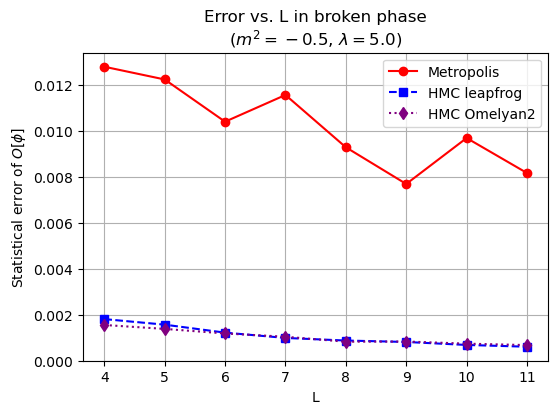
\includegraphics[width=\linewidth]{images/error_Python_broken.png}
        \caption{Broken phase with negative mass}
        \label{fig:broken_python_errors}
    \end{subfigure}
    \hfill 
    \begin{subfigure}[b]{0.48\linewidth}
        \centering
        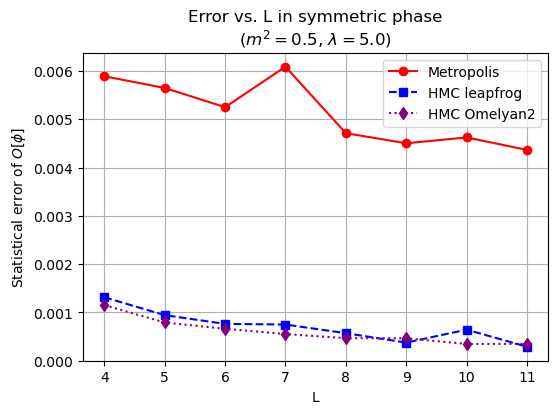
\includegraphics[width=\linewidth]{images/error_Python_symmetric.png}
        \caption{Symmetric phase with positive mass}
        \label{fig:symmetric_python_errors}
    \end{subfigure}
    \caption{Statistical errors as a function of lattice size $L$ for the broken and symmetric phase, algorithms in Python.}
    \label{fig:python_errors}
\end{figure}
The following Figure \ref{fig:rust_errors} shows the statistical errors of both phases resulting from the Rust implemented algorithms.
\begin{figure}[H]
    \centering
    \begin{subfigure}[b]{0.48\linewidth}
        \centering
        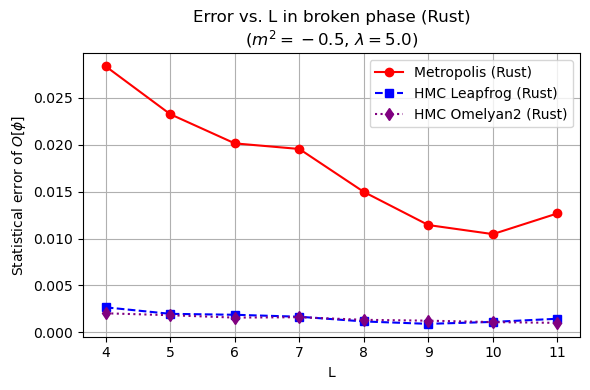
\includegraphics[width=\linewidth]{images/error_Rust_broken.png}
        \caption{Broken phase with negative mass}
        \label{fig:broken_rust_errors}
    \end{subfigure}
    \hfill 
    \begin{subfigure}[b]{0.48\linewidth}
        \centering
        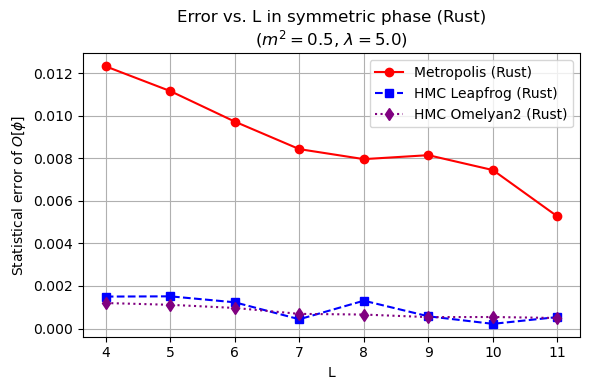
\includegraphics[width=\linewidth]{images/error_Rust_symmetric.png}
        \caption{Symmetric phase with positive mass}
        \label{fig:symmetric_rust_errors}
    \end{subfigure}
    \caption{Statistical Errors as a function of lattice size $L$ for the broken and symmetric phase, algorithms in Rust.}
    \label{fig:rust_errors}
\end{figure}
\subsubsection*{Comments on the Results}
\begin{itemize}
    \item In both the symmetric and broken phases with both Python and Rust, the Metropolis produces significantly larger statistical errors than the HMC algorithm. The HMC algorithm has similar statistical errors for the two different integrators leapfrog and omelyan2. 
    \item For both versions of HMC, the Python and Rust implementations have similar statistical errors. The statistical error of the Metropolis algorithm is approximately twice as large as in the Rust version, for unknown reasons.
    \item In the broken phase the statistical error is significantly larger than in the symmetric phase. This is a consequence of the presence of two degenerate vacua, between which the Monte Carlo simulation can tunnel. These tunneling events lead to long autocorrelation times and large fluctuations of observables, thereby increasing the statistical uncertainty. In contrast, the symmetric phase contains a single stable vacuum and exhibits faster decorrelation.
    \item In all simulations, the statistical error decreases with increasing lattice size $L$. Most likely, this behaviour can be attributed to how the average is computed. The measured observables are spatial averages over the lattice, their variance decreases as $1/V = 1/L^2$. Although autocorrelation times increase with lattice size, especially in the broken phase, the reduction of statistical fluctuations due to averaging over more degrees of freedom dominates in the parameter range considered.
\end{itemize}
\subsection{Autocorrelations}
Autocorrelations measure the memory of a Markov chain and quantify the dependence of successive configurations. High autocorrelation reduces the effective number of independent samples, increasing statistical errors. We discuss the computation of integrated autocorrelation times and their impact on the precision of measured observables.\\\\
The following Figure \ref{fig:autocorr_python} shows the integrated autocorrelation time as a function of lattice size $L$ for the different algorithms implemented in Python. 
\begin{figure}[H]
    \centering
    \begin{subfigure}[b]{0.48\linewidth}
        \centering
        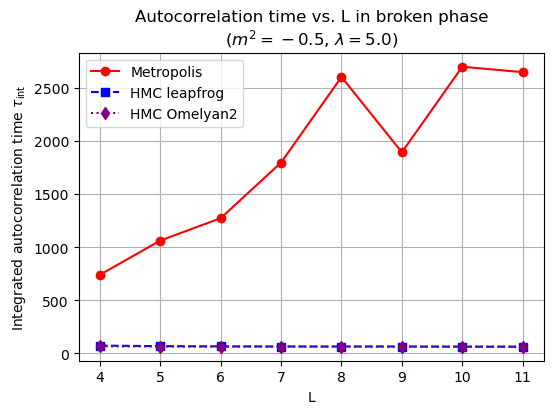
\includegraphics[width=\linewidth]{images/autocorr_Python_broken.png}
        \caption{Broken phase with negative mass}
        \label{fig:broken_python_autocorr}
    \end{subfigure}
    \hfill 
    \begin{subfigure}[b]{0.48\linewidth}
        \centering
        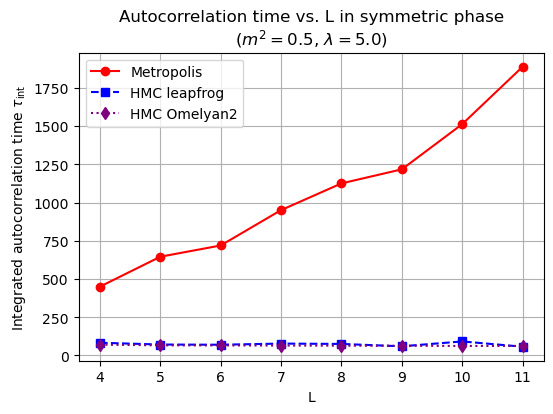
\includegraphics[width=\linewidth]{images/autocorr_Python_symmetric.png}
        \caption{Symmetric phase with positive mass}
        \label{fig:symmetric_python_autocorr}
    \end{subfigure}
    \caption{Autocorrelations as a function of lattice size $L$ for the broken and symmetric phase, algorithms in Python.}
    \label{fig:autocorr_python}
\end{figure}
The following Figure \ref{fig:autocorr_rust} shows the integrated autocorrelation time as a function of lattice size $L$ for the different algorithms implemented in Rust. 
\begin{figure}[H]
    \centering
    \begin{subfigure}[b]{0.48\linewidth}
        \centering
        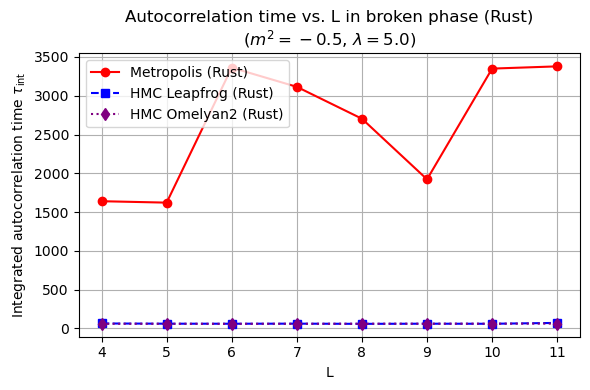
\includegraphics[width=\linewidth]{images/autocorr_Rust_broken.png}
        \caption{Broken phase with negative mass}
        \label{fig:broken_rust_autocorr}
    \end{subfigure}
    \hfill 
    \begin{subfigure}[b]{0.48\linewidth}
        \centering
        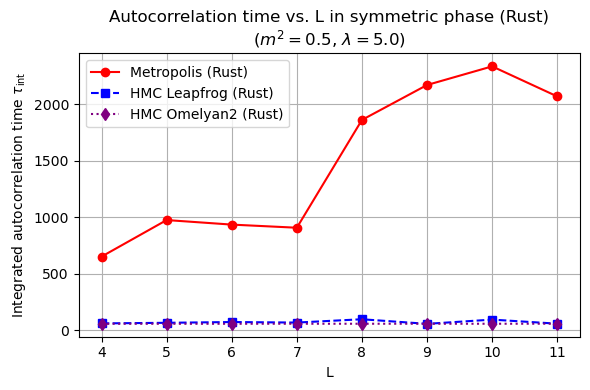
\includegraphics[width=\linewidth]{images/autocorr_Rust_symmetric.png}
        \caption{Symmetric phase with positive mass}
        \label{fig:symmetric_rust_autocorr}
    \end{subfigure}
    \caption{Autocorrelations as a function of lattice size $L$ for the broken and symmetric phase, algorithms in Rust.}
    \label{fig:autocorr_rust}
\end{figure}
\subsubsection*{Comments on the Results}
\begin{itemize}
    \item In all panels, for both Rust and Python, the integrated autocorrelation time increases with lattice size $L$, as expected. This is a manifestation of critical slowing down. As the correlation length grows with the system size, local update algorithms require more steps to decorrelate configurations. The effect is visible for Metropolis, for HMC it is strongly suppressed (since the updates are not local).
    \item The Metropolis algorithm has very large autocorrelation times, which tend to grow with the lattice size $L$. The autocorrelation times for the broken phase are larger, which is expected. In the broken phase, the system has two degenerate minima, local Metropolis updates struggle to tunnel between them. Metropolis becomes impractical for large systems, especially in the broken phase. 
    \item Both HMC variants show dramatically reduced autocorrelation times, nearly flat at $L$. Omelyan2 is systematically slightly lower, since its integration error is smaller. This shows that HMC avoids critical slowing down effectively. Global molecular-dynamics updates decorrelate the system much faster than local update proposals. 
    \item The comparison of the broken and symmetric phase reveals that the broken phase (negative mass square) has larger autocorrelation times overall. The physical reason for that is that the potential has two minima and the configurations must tunnel between two vacua. Metropolis has local updates and therefore almost never tunnels, which leads to large autocorrelation times. HMC tunnels quite efficiently, but still shows a slightly increased autocorrelation. 
    \item When comparing the results from the Rust and Python implementations, the HMC results match mostly. However, there are some discrepancies for the Metropolis algorithm of unknown cause. The physics are expected to be independent of the implementation. Differences could be due to floating-point accumulation order, random number generator differences or a mistake in one of the implementations. The cause could not be identified so far, this needs further investigations.  
\end{itemize}
\section{Comparison of Integrators}\label{sec: int_comparison}
This section contains the result of the analysis comparing the leapfrog and the omelyan2 integrators, which have been described in Chapter \ref{sec: integrators}. 
\subsection{HMC Energy Violations for Symmetric and Broken Phases}
The HMC simulation (Python version only) was run for two phases: the symmetric phase ($m^2 = 0.5$) and the broken phase $(m^2 = -0.5)$, using both the leapfrog and omelyan2 integrators. For each phase, 2000 HMC trajectories on a lattice of size $L = 8$ were computed, using $\varepsilon = 0.1$. \\\\
For each trajectory, we recorded the change in the Hamiltonian between the initial and final configurations. This measures energy conservation of the integrator and is directly related to the HMC acceptance probability.\\\\
The following Table \ref{tab: deltaH_statistics} shows the means and standard deviations of $\Delta H$ for each integrator and for each phase. 
\begin{table}[H]
\centering
\begin{tabular}{lcc}
\hline
\textbf{Phase and Integrator} & \textbf{Mean($\Delta H$)} & \textbf{Std($\Delta H$)} \\
\hline
\textbf{Symmetric Phase} & & \\
\quad Leapfrog & $-3.753\times 10^{-3}$ & $7.684\times 10^{-2}$ \\
\quad Omelyan2 & $-2.297\times 10^{-5}$ & $1.559\times 10^{-3}$ \\
\hline
\textbf{Broken Phase} & & \\
\quad Leapfrog & $-3.252\times 10^{-3}$ & $6.990\times 10^{-2}$ \\
\quad Omelyan2 & $8.146\times 10^{-6}$ & $2.743\times 10^{-3}$ \\
\hline
\end{tabular}
\caption{Statistics of Hamiltonian differences $\Delta H$ for symmetric and broken phases using Leapfrog and Omelyan2 integrators.}
\label{tab: deltaH_statistics}
\end{table}
The following Figures \ref{fig:symmetric_hists} and \ref{fig:broken_hists} show the energy violation distributions for both integrators in the symmetric and broken phase. The scatter plots display $\Delta H$ for each trajectory. 
\begin{figure}[H]
    \centering
    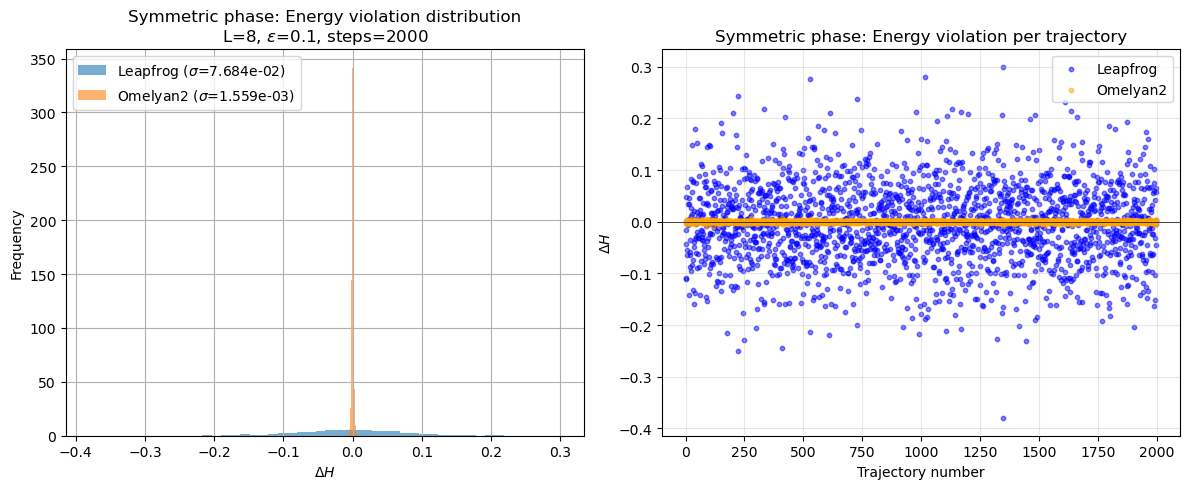
\includegraphics[width=\linewidth]{images/symmetric_hists.png}
    \caption{Distribution of $\Delta H = H_{\text{old}} - H_{\text{new}}$ in the symmetric phase.}
    \label{fig:symmetric_hists}
\end{figure}
\begin{figure}[H]
    \centering
    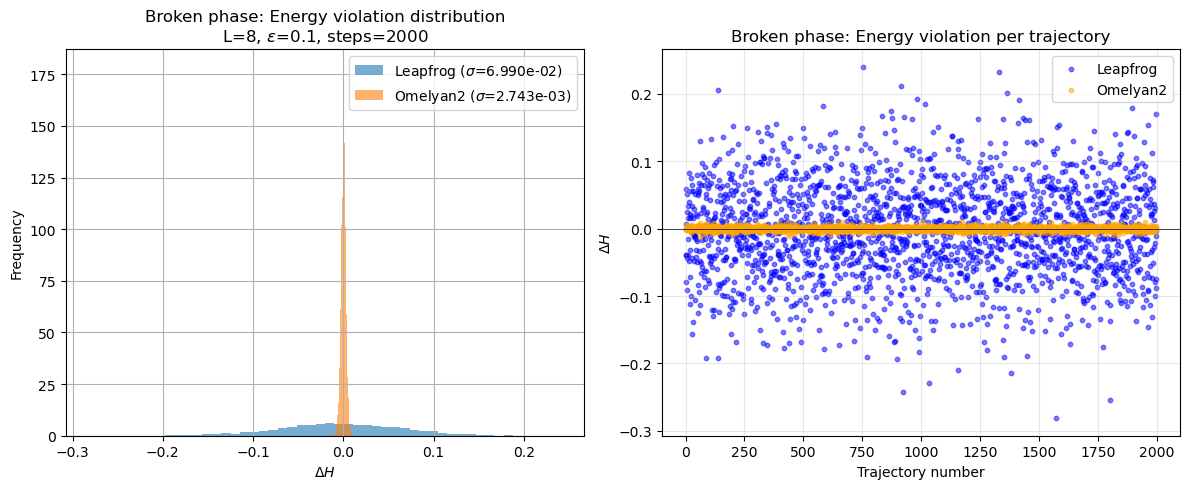
\includegraphics[width=\linewidth]{images/broken_hist.png}
    \caption{Distribution of $\Delta H = H_{\text{old}} - H_{\text{new}}$ in the broken phase.}
    \label{fig:broken_hists}
\end{figure}
\subsubsection*{Comments on the Results}
\begin{itemize}
    \item It is clearly visible in both phases that omelyan2 produces smaller $\Delta H$ fluctuations than leapfrog, indicating better energy conservation.
    \item Leapfrog shows wider distributions and occasional large violations, which could lead to reduced accpetance rate in HMC algorithm.
    \item The difference between symmetric and broken phases is minor, but the analysis confirms the robustness of omelyan2 across different physical regimes.
\end{itemize}
\subsection{Influence of Step Size \texorpdfstring{$\varepsilon$}{eps}}
The HMC simulations were repeated with different step sizes $\varepsilon$. The following Figure \ref{fig:stepsize_comparison} shows the standard deviation of $\Delta H$ as a function of stepsize $\varepsilon$ in both phases and for both leapfrog and omelyan2. 
\begin{figure}[H]
    \centering
    \begin{subfigure}[b]{0.48\linewidth}
        \centering
        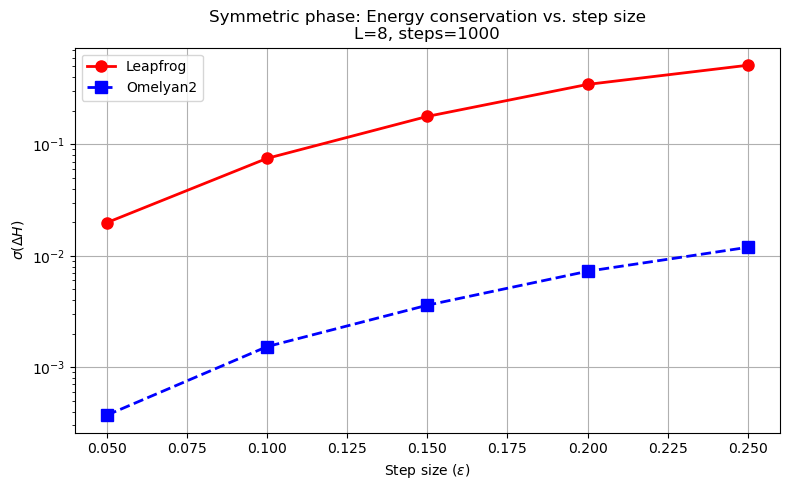
\includegraphics[width=\linewidth]{images/symmetric_stepsize.png}
        \caption{Symmetric phase.}
        \label{fig:symmetric_stepsize}
    \end{subfigure}
    \hfill 
    \begin{subfigure}[b]{0.48\linewidth}
        \centering
        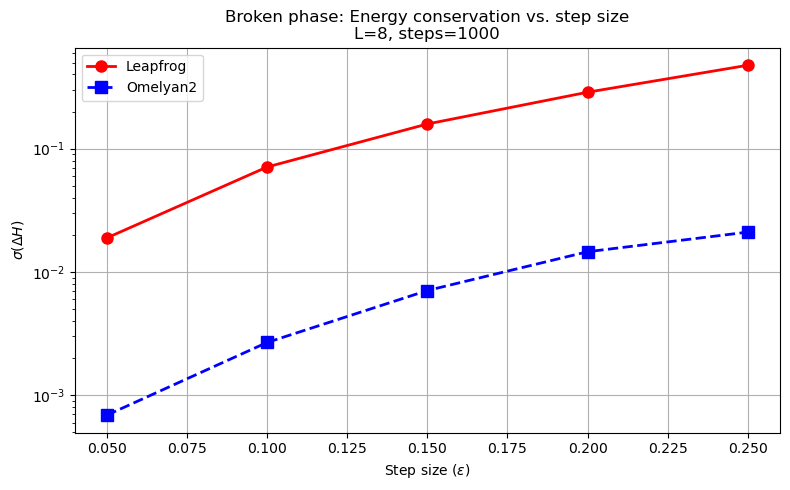
\includegraphics[width=\linewidth]{images/broken_stepsize.png}
        \caption{Broken phase.}
        \label{fig:broken_stepsize}
    \end{subfigure}
    \caption{Standard deviation of $\Delta H$ as a function of stepsize $\varepsilon$. Note that the scale is logarithmic.}
    \label{fig:stepsize_comparison}
\end{figure}
\subsubsection*{Comments on the Results}
\begin{itemize}
    \item There is the expected dependence of $\sigma(\Delta H)$ on the stepsize $\varepsilon$, the standard deviation grows with growing stepsize. 
    \item Both integrators show similar scaling with $\varepsilon$, although omelyan2 maintains consistently lower $\sigma(\Delta H)$ than leapfrog.
    \item The difference between the two phases is minor, indicating that the integrator performance is independent of the physical regime for our parameter choices.
\end{itemize}
\section{Results with the Topological Charge}\label{sec: top_charge_results}
This section is based on \cite{De_2005}. The Metropolis algorithm (Rust version) was used, since it has been extendend to include the option of aperiodic boundary conditions. \\
To study the behaviour of the topological charge as a function of the lattice size, simulations were performed using the Metropolis algorithm for both periodic (PBC) and anti-periodic (APBC) boundary conditions. The number of steps has been increased to $83'160$ (highly composite number, see \cite{wikipedia_highly_composite_number}) to obtain better statistic and clearer results.\\\\
Figure \ref{fig:top_charge} shows the measured topological charge $Q_R$ as a function of the lattice size $L$ for both the broken and symmetric phases, obtained using the Metropolis algorithm with periodic (PBC) and anti-periodic (APBC) boundary conditions. The quantity $Q_R$ measures the difference in topology induced by changing the boundary conditions, and therefore serves as a probe of non-trivial field configurations such as kinks and anti-kinks, see Section \ref{sec:topology}.
\begin{figure}[H]
    \centering
    \begin{subfigure}[b]{0.48\linewidth}
        \centering
        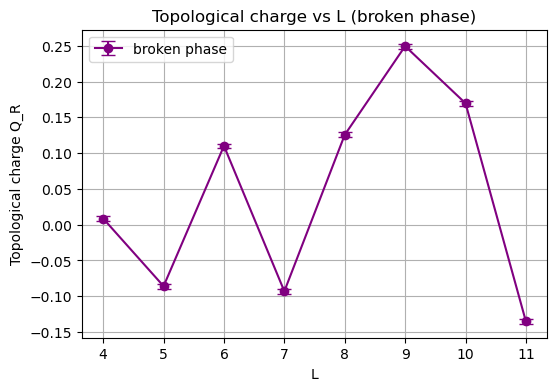
\includegraphics[width=\linewidth]{images/top_charge_broken.png}
        \caption{Topological charge $Q_R$ in the broken phase}
        \label{fig:top_charge_broken}
    \end{subfigure}
    \hfill 
    \begin{subfigure}[b]{0.48\linewidth}
        \centering
        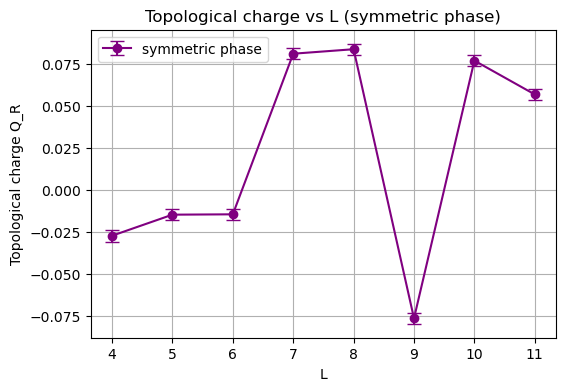
\includegraphics[width=\linewidth]{images/top_charge_symmetric.png}
        \caption{Topological charge $Q_R$ in the symmetric phase}
        \label{fig:top_charge_symmetric}
    \end{subfigure}
    \caption{Topological charge $Q_R$ as a function of lattice size $L$ for the broken and symmetric phases, using PBC and APBC.}
    \label{fig:top_charge}
\end{figure}
\subsubsection*{Comments on the Results}
\begin{itemize}
    \item In the broken phase, the scalar potential possesses two degenerate minima, allowing for topological non-trivial field configurations. This is reflected in the results, $Q_R$ fluctuates around non-zero values, which indicates topological excitations. The sign changes reflect tunneling between the vacua. The magnitude of $Q_R$ is clearly larger than in the symmetric phase. We observe no dependence on the lattice size $L$. 
    \item In the symmetric phase, the potential has one minimum and topological effects are suppressed. This is cleary visible, the fluctuations have a much smaller magnitude and are close to zero. The fluctuations can likely be explained by statistical noise. 
    \item Overall, the behaviour of $Q_R$ in both phases agrees with the expectations of $\phi^4$ theory. Nontrivial topological structures appear only when degenerate minima exist (broken phase), and vanish in the symmetric phase.
\end{itemize}